\documentclass[10pt]{article}

% ============================================================
% ARES - IREC 2027 SUBMISSION-STYLE WORKING DRAFT
% Structured to match the 2026 IREC technical-report requirements.
% Final typography must be checked against the 2027 ESRA template.
% ============================================================

\usepackage[margin=0.72in]{geometry}
\usepackage{graphicx}
\usepackage{booktabs}
\usepackage{tabularx}
\usepackage{array}
\usepackage{multirow}
\usepackage{longtable}
\usepackage{siunitx}
\usepackage{amsmath}
\usepackage{enumitem}
\usepackage{caption}
\usepackage{hyperref}
\usepackage{xcolor}
\usepackage{microtype}
\usepackage{tikz}
\usetikzlibrary{arrows.meta,positioning,shapes.geometric,calc}

\setlength{\parindent}{0.18in}
\setlength{\parskip}{0.15em}
\setlength{\textfloatsep}{8pt plus 2pt minus 2pt}
\setlength{\floatsep}{7pt plus 2pt minus 2pt}
\setlength{\intextsep}{7pt plus 2pt minus 2pt}
\setlist[itemize]{nosep,leftmargin=0.22in}
\setlist[enumerate]{nosep,leftmargin=0.25in}
\captionsetup{font=small,skip=4pt}
\hypersetup{colorlinks=true,linkcolor=black,citecolor=black,urlcolor=blue}
\sisetup{detect-all=true}

\newcommand{\ARES}{A.R.E.S.}
\newcommand{\COMET}{C.O.M.E.T.}
\newcommand{\DEIMOS}{D.E.I.M.O.S.}
\newcommand{\PHOBOS}{P.H.O.B.O.S.}
\newcommand{\TBD}{\textbf{TBD}}

\newcommand{\status}[1]{\textit{#1}}
\newcommand{\req}[1]{\textbf{#1}}

\begin{document}

% ============================================================
% TITLE / AUTHOR BLOCK
% ============================================================
\begin{center}
{\LARGE\bfseries A.R.E.S.: Aurora Rocket and Experimental Systems}\\[4pt]
{\large Team ID Pending Assignment -- Project Technical Report to the 2027 IREC}\\[8pt]
Nicholas Krupa, Kyle Eckert, Liam Gordon\\
University of Hartford, West Hartford, Connecticut, USA\\
Faculty Advisors: Paul Slaboch and Enrico Obst\\
Level 3 Mentor: Richard Comshaw\\[4pt]
\textit{Working submission draft based on the 2026 IREC Rules \& Requirements and DTEG. Update against the 2027 documents when released.}
\end{center}

\vspace{0.08in}
\hrule
\vspace{0.12in}

% ============================================================
% EXECUTIVE SUMMARY - 2026 limit: 1 page
% ============================================================
\section*{Executive Summary}

The University of Hartford AURORA team is developing \ARES{}, a single-stage, 6-inch-class fiberglass sounding rocket for the IREC 10,000-ft COTS category. The current vehicle is approximately \SI{3.71}{m} (146 in) long with a \SI{156.7}{mm} maximum airframe outside diameter, three aft G10 fiberglass fins, four forward canards, a \SI{75}{mm} motor mount, redundant dual-event recovery, and a removable experimental payload. The baseline motor is the AeroTech N2700W-PS, a commercial \SI{10322}{N.s} N-class motor using RMS-75/10240 hardware.

The latest stored OpenRocket run predicts an apogee of \SI{3002.5}{m} AGL (9,850.6 ft), maximum velocity of \SI{299.76}{m/s} (Mach 0.887), maximum acceleration of 12.26 g, and a full-rail exit velocity of \SI{34.35}{m/s} using a \SI{5.18}{m} (17 ft) 1515 rail. A current component-by-component mass accounting of the serialized OpenRocket model gives an estimated launch mass of approximately \SI{28.79}{kg} (63.47 lb), including the loaded N2700. Using the current \SI{0.807}{m} rail-button spacing, the corresponding ESRA effective-rail departure velocity is preliminarily estimated at approximately \SI{31.6}{m/s}; the final application value will be exported from a no-wind OpenRocket run using the final CG/CP configuration.

Recovery uses a 36-in Fruity Chutes compact elliptical drogue at apogee and a 120-in Fruity Chutes Iris main at \SI{200}{m} AGL. The redundant deployment paths are a student-developed \COMET{} flight computer and a PerfectFlite StratoLoggerCF COTS dual-deployment computer, with independent switches, power, sensing, energetics, and initiators. A Featherweight Blue Raven 2 is the working COTS official-altitude logger. Recovery tracking is assigned to an Altus Metrum TeleGPS v4.0 COTS GPS tracker operating in the IREC-assigned 70-cm channel plan. Competition power will use mechanically restrained cylindrical metal-cased Li-ion cells; no LiPo pouch batteries are part of the baseline.

The official competition payload is \PHOBOS{}, a removable approximately \SI{2}{kg} phased-array communications experiment. \DEIMOS{} is separate launch-vehicle experimental telemetry/orientation avionics. The four-canard roll-control system is an optional experiment, not a flight requirement: ARES will remain passively stable and recover nominally with active control disabled. The canards are commanded to a mechanically neutral condition for restricted boost and on abort, loss of control power, invalid sensor state, or excessive attitude. Qualification will include structural analysis, no-wind stability, fin flutter, full-scale recovery pop tests, independent recovery-electronics tests, battery endurance, COTS/experimental RF range tests, phased-array laboratory characterization, active-control fail-safe tests, and a full-scale spring qualification flight.

% ============================================================
% 1. INTRODUCTION - 2026 limit: 2 pages
% ============================================================
\section{Introduction}

\subsection{Competition Category and Mission}
ARES is being prepared for the IREC 10,000-ft COTS solid-motor category. This is AURORA's first IREC entry, and the team selected 10K COTS deliberately: the group already has substantial COTS high-power flight experience and a mature 75-mm fiberglass vehicle architecture, while the category allows qualification effort to remain focused on recovery, avionics, payload, and optional control research rather than adding SRAD propulsion risk. The mission is to launch a removable functional payload to approximately \SI{10000}{ft} AGL, recover the vehicle under redundant dual-event recovery, and return usable flight, payload, and telemetry data.

\subsection{Program Goals and Distinguishing Features}
The project has four technical goals: (1) produce a robust 6-inch fiberglass launch vehicle that can repeatedly support N-class flight; (2) qualify a student-developed flight computer while retaining independent COTS recovery; (3) fly a removable functional RF payload meeting the IREC payload-mass requirement; and (4) investigate active roll-control hardware without making vehicle stability dependent on active control. The design deliberately separates competition-critical functions from experimental functions: loss of \PHOBOS{}, \DEIMOS{}, or active roll control shall not prevent stable flight or nominal recovery.

\subsection{Academic Program, Team Experience, and Contributors}
ARES is a University of Hartford senior capstone project conducted through the College of Engineering, Technology, and Architecture and AURORA (Advanced Undergraduate Rocketry Operations and Research Association). Nicholas Krupa leads systems integration, \DEIMOS{}, roll control, and co-develops \COMET{}; Kyle Eckert leads \PHOBOS{} and co-develops \COMET{}; Liam Gordon leads mechanical design, structural integration, and ANSYS-based loading analysis. Paul Slaboch and Enrico Obst advise the project. Ensign-Bickford Aerospace \& Defense supports the broader capstone effort, and NASA Connecticut Space Grant supports phased-array development.

AURORA currently has nine members certified NAR Level 1 or higher; two currently hold Level 2 and three additional members are pursuing Level 2 during Fall 2026. Nicholas Krupa is pursuing Level 3 certification in Spring 2027. His 6.5-ft-long, 4-in-diameter fiberglass Level 2 vehicle has flown twice at the Champlain Region Model Rocketry Club on an AeroTech K850, and the team has flown two additional Level-2-class vehicles to test custom dual-deployment avionics. AURORA has received multiple NASA Connecticut Space Grant undergraduate research/project awards during the last three years, including current support associated with ARES.

Richard Comshaw serves as the current Level 3 mentor. He is an experienced high-power rocketeer active with METRA and regularly supports NAR certification activity. His role is to review the N-class vehicle design, recovery architecture, manufacturing decisions, qualification testing, and launch readiness. Current ESRA guidance for the 2027 cycle shifts the application requirement from naming a Flyer of Record (FoR) to identifying committed mentors; the FoR is designated later in the season. A qualified FoR will therefore be confirmed on the 2027 schedule rather than treated as an unresolved application field.

\begin{table}[ht]
\centering
\caption{Current team responsibility split.}
\begin{tabularx}{\linewidth}{@{}lX@{}}
\toprule
\textbf{Member} & \textbf{Primary responsibility} \\
\midrule
Nicholas Krupa & Systems integration; \DEIMOS{}; active roll control; \COMET{}; recovery integration \\
Kyle Eckert & \PHOBOS{} phased-array payload; \COMET{}; RF/electrical integration \\
Liam Gordon & Airframe/mechanical integration; structural analysis; manufacturing drawings \\
\bottomrule
\end{tabularx}
\end{table}

\subsection{Management and Report Preparation}
Subsystem owners maintain CAD, schematics, code, calculations, test records, and interface requirements for their hardware. Changes affecting mass, CG, recovery, propulsion, or external geometry are propagated to the integrated OpenRocket/CAD baseline before flight decisions are made. Report sections are drafted by the responsible subsystem owner and consolidated by the systems lead. This document is intentionally organized around the IREC-required report structure; detailed evidence is moved to Appendices A--F rather than repeated in the main body.

\subsection{Program Continuity and Competition Logistics}
ARES will be built and flight-tested in Spring 2027 regardless of IREC selection because it is the team's senior capstone vehicle. AURORA is also in its third consecutive year participating in NASA RockSat-C, which has required repeated travel with flight hardware to Wallops Island, Virginia. The working IREC logistics plan is to transport the rocket and non-energetic ground hardware by road to Midland, Texas; reserve lodging after the November acceptance announcement; and use existing EBAD project support supplemented, if required, by a NASA Connecticut Space Grant travel-grant application. The current minimum student travel party is the three capstone students. Flyer-of-Record attendance will be added once that role is designated; mentor attendance is not assumed unless the mentor and FoR are the same person.

% ============================================================
% 2. SYSTEM ARCHITECTURE
% ============================================================
\section{System Architecture Overview}

\subsection{Integrated Vehicle}
The current configuration is a \SI{3.71}{m} long G12 fiberglass vehicle with a 30-in ogive nose, multiple 6-in-class body sections/couplers, a removable \PHOBOS{} payload, forward experimental avionics, dual-event recovery, a central avionics bay, a forward canard module, and a 60-in aft fin can containing the \SI{75}{mm} motor mount. Figure~\ref{fig:architecture} shows the current top-level physical architecture.

\begin{figure}[ht]
\centering
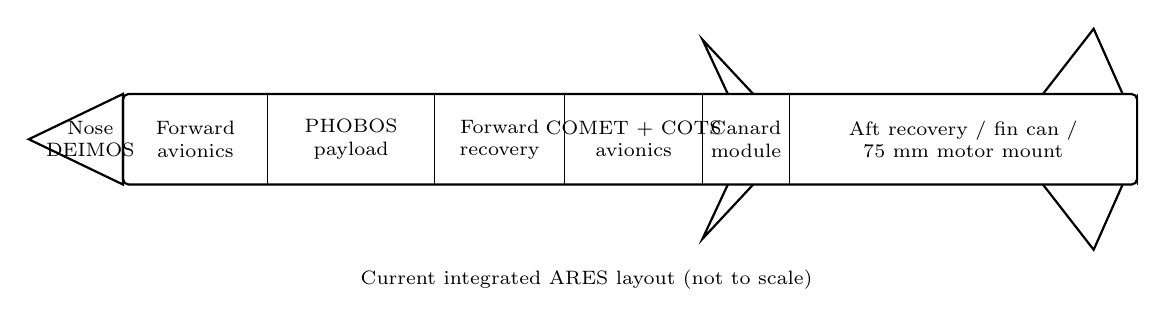
\begin{tikzpicture}[x=0.92cm,y=0.92cm,>=Latex,font=\scriptsize]
  % body
  \draw[thick,rounded corners=2pt] (0,0) rectangle (14,1.25);
  \draw[thick] (-1.3,0.625) -- (0,0) -- (0,1.25) -- cycle;
  % section dividers
  \foreach \x in {2.0,4.3,6.1,8.0,9.2,14.0} {\draw (\x,0)--(\x,1.25);}
  % labels
  \node[align=center] at (-0.45,0.625) {Nose\\DEIMOS};
  \node[align=center] at (1.0,0.625) {Forward\\avionics};
  \node[align=center] at (3.15,0.625) {PHOBOS\\payload};
  \node[align=center] at (5.2,0.625) {Forward\\recovery};
  \node[align=center] at (7.05,0.625) {COMET + COTS\\avionics};
  \node[align=center] at (8.6,0.625) {Canard\\module};
  \node[align=center] at (11.6,0.625) {Aft recovery / fin can /\\75 mm motor mount};
  % canards/fins
  \draw[thick] (8.35,1.25)--(8.0,2.0)--(8.7,1.25);
  \draw[thick] (8.35,0)--(8.0,-0.75)--(8.7,0);
  \draw[thick] (12.7,1.25)--(13.4,2.15)--(13.8,1.25);
  \draw[thick] (12.7,0)--(13.4,-0.9)--(13.8,0);
  \node[below] at (6.4,-1.05) {Current integrated ARES layout (not to scale)};
\end{tikzpicture}
\caption{Top-level integrated launch-vehicle architecture. Final report will replace this schematic with the revision-controlled vehicle cutaway.}
\label{fig:architecture}
\end{figure}

\begin{table}[ht]
\centering
\caption{Current vehicle baseline.}
\begin{tabularx}{\linewidth}{@{}l l X@{}}
\toprule
\textbf{Parameter} & \textbf{Current value} & \textbf{Basis} \\
\midrule
Stages & 1 & Single-stage COTS solid \\
Overall length & 146 in / 3.71 m & Current OpenRocket geometry \\
Airframe OD & 6.17 in / 156.7 mm & Madcow FT60 G12 tube \\
Aft fins & 3 & 0.250-in G10, through-the-wall \\
Canards & 4 & 0.250-in G10, neutral for passive flight \\
Motor mount & 75 mm & Approx. 48-in fiberglass tube \\
Launch guide & 1515, 17 ft assumed & IREC single-stage solids baseline \\
Drogue / main & 36 in / 120 in & Fruity Chutes \\
Official payload & \PHOBOS{}, approx. 2.0 kg minimum & Removable for independent weigh-in \\
\bottomrule
\end{tabularx}
\end{table}

\subsection{Aerostructures and Stability}
The primary airframe is filament-wound G12 fiberglass. The current five external G12 tube mass overrides are 1.134, 0.170, 1.701, 0.170, and \SI{3.402}{kg}; these use the manufacturer's nominal \SI{24}{oz/ft} tube weight and replace lighter density-only estimates. The fin can uses three \SI{6.69}{in} semi-span, \SI{23.72}{in} root-chord, \SI{3.94}{in} tip-chord, \SI{0.250}{in} G10 fins. Final fin-tab geometry, fillet mass, and local reinforcement will follow the manufacturing CAD.

The 2026 DTEG required subsonic vehicles to maintain at least 7.5\% of vehicle length as static margin through first recovery deployment, with maximum stability of 18\% at launch and 25\% in flight. For the present \SI{146}{in} / \SI{6.17}{in} geometry these correspond to approximately 1.77 calibers minimum, 4.26 calibers maximum at launch, and 5.92 calibers maximum in flight. A no-wind stability-versus-time result is still required from the final mass model. Because the latest maximum simulated speed is \SI{299.76}{m/s}, the 2026 fin-flutter criterion would require demonstrated flutter velocity of at least approximately \SI{449.6}{m/s}. Final structural substantiation will report fin shear modulus, predicted flutter velocity, axial/bending loads, and safety factors.

The launch-guidance hardware uses two 1515 rail buttons attached through reinforced hard points with metallic fasteners. The exact axial locations will be frozen with the internal structural CAD. Adhesive-only attachment is not used. The design will be checked for horizontal underslung loading on the rail and for unobstructed access to avionics arming controls.

\subsection{Propulsion Subsystem}
The baseline propulsion system is the AeroTech N2700W-PS in RMS-75/10240 hardware. The motor is commercially manufactured and therefore satisfies the intended COTS category definition. Manufacturer data used in the current analysis are summarized in Table~\ref{tab:motor}.

\begin{table}[ht]
\centering
\caption{AeroTech N2700W-PS baseline data.}
\label{tab:motor}
\begin{tabular}{@{}ll@{}}
\toprule
Motor designation & N2700W-PS, 75 mm \\
Total impulse & 10,322 N\,s \\
Average thrust & approx. 2,717 N \\
Peak thrust & approx. 4,625 N \\
Burn time & approx. 3.8 s \\
Propellant mass & 5.275 kg \\
Loaded motor mass & 9.058 kg \\
Overall motor length & approx. 48.5 in \\
Hardware & RMS-75/10240 \\
\bottomrule
\end{tabular}
\end{table}

Motor thrust is reacted through a 6-in/75-mm aluminum thrust plate and internal fiberglass structure. The current model includes the thrust plate as a separate \SI{0.350}{kg} aft mass and the AeroPack 75-mm flanged retainer as a separate \SI{0.139}{kg} mass. Final design verification will check local bearing, fastener, plate, centering-ring, and all-thread loads against the N2700 thrust history and handling loads.

\subsection{Avionics}
ARES separates competition-critical recovery from experimental avionics. The primary student-developed computer is \COMET{}, an SRAD flight computer using barometric and inertial sensing, independent drogue/main outputs, continuity monitoring, battery monitoring, flash logging, external arming/status, and telemetry interfaces. \COMET{} is paired with a PerfectFlite StratoLoggerCF as the independent COTS dual-deployment path. Each recovery path will use its own arming device, battery, sensing/computer, deployment output, charge, and initiator. A dual-pole common switch is not used as a substitute for independent arming.

The Featherweight Blue Raven 2 is the current COTS official-altitude logger and an additional independent recorded data source. Required recovery tracking is assigned to an Altus Metrum TeleGPS v4.0, a current-production COTS GPS tracker/logger using a 70-cm telemetry link, u-blox MAX-M10S receiver, and onboard flash logging. The tracker will use the IREC-assigned frequency and a separately switched/powered 3.7-V cylindrical metal-cased Li-ion supply qualified by bench test. Operation on 70 cm requires an appropriately licensed control operator. All safety-critical wiring will be mechanically retained, strain-relieved, labeled, and supported; daughterboards will not rely on electrical connectors as structural supports.

The competition battery baseline is rechargeable Li-ion power assembled from cylindrical metal-cased cells in restrained packs. LiPo pouch batteries are excluded. Each competition-critical recovery path has a separate power source. Battery capacity will be verified by measured current draw and endurance testing with margin for pad delays.

\begin{figure}[ht]
\centering
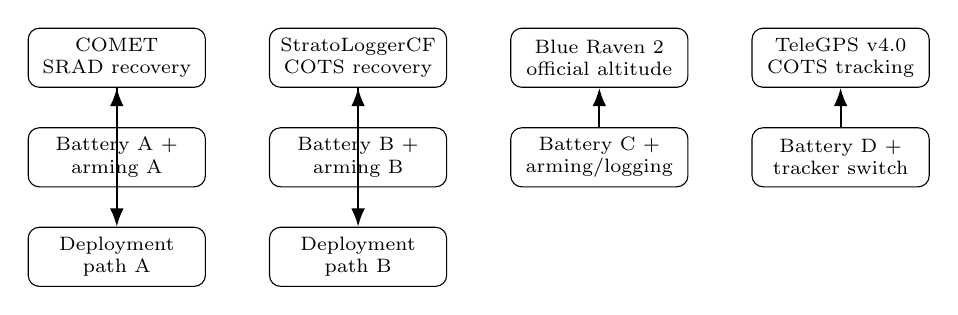
\begin{tikzpicture}[node distance=5mm and 8mm,font=\scriptsize,
box/.style={draw,rounded corners,align=center,minimum width=2.25cm,minimum height=0.75cm},
arr/.style={-Latex,thick}]
\node[box] (comet) {COMET\\SRAD recovery};
\node[box,right=of comet] (sl) {StratoLoggerCF\\COTS recovery};
\node[box,right=of sl] (br) {Blue Raven 2\\official altitude};
\node[box,right=of br] (gps) {TeleGPS v4.0\\COTS tracking};
\node[box,below=of comet] (bat1) {Battery A +\\arming A};
\node[box,below=of sl] (bat2) {Battery B +\\arming B};
\node[box,below=of br] (bat3) {Battery C +\\arming/logging};
\node[box,below=of gps] (bat4) {Battery D +\\tracker switch};
\node[box,below=of bat1] (py1) {Deployment\\path A};
\node[box,below=of bat2] (py2) {Deployment\\path B};
\draw[arr] (bat1)--(comet); \draw[arr] (bat2)--(sl); \draw[arr] (bat3)--(br); \draw[arr] (bat4)--(gps);
\draw[arr] (comet)--(py1); \draw[arr] (sl)--(py2);
\end{tikzpicture}
\caption{Working competition-critical avionics partition. Recovery paths A/B are independent; the official-altitude logger and required COTS GPS tracker are separately powered and switched.}
\label{fig:avionics}
\end{figure}

\subsection{Recovery Subsystem}
ARES uses dual-event parachute recovery. The 36-in Fruity Chutes compact elliptical drogue is deployed at apogee; the 120-in Fruity Chutes Iris main is commanded at \SI{200}{m} (656 ft) AGL. The current model uses \(C_D=1.55\) and \SI{0.0936}{kg} for the drogue and \(C_D=2.2\) and \SI{0.6237}{kg} for the main. Two 25-ft 1/4-in tubular Kevlar harnesses are the current baseline. Load-bearing recovery links will be closed forged steel or stainless-steel hardware. The main and drogue will use contrasting visible colors.

The current stored deployment-velocity metric is \SI{19.55}{m/s}; if a clean rerun confirms this is the drogue descent rate at main deployment, it is slightly below the 2026 target range of \SIrange{20}{40}{m/s} and will require adjustment. The current stored landing velocity is \SI{5.19}{m/s}, below the 2026 \SI{11}{m/s} maximum. Final recovery analysis will use the IREC-prescribed launch-site elevation and the final vehicle mass. Charge mass, shear-pin count, packed configuration, separation distance, and opening loads will be established by ground testing rather than simulation alone.

\subsection{Telemetry and Tracking}
Required recovery tracking is provided by the Altus Metrum TeleGPS v4.0 COTS tracker on the IREC-assigned 70-cm channel. It is independent of both recovery computers and of the research telemetry systems. \DEIMOS{} remains experimental launch-vehicle telemetry/orientation avionics with sub-\SI{200}{g} mass target, IMU/GPS/barometric sensing, 915-MHz LoRa telemetry, approximately 20-Hz update rate, at least \SI{4}{km} experimental range, and onboard flash logging.

The RF architecture is intentionally partitioned: TeleGPS is required COTS recovery tracking; \DEIMOS{} is experimental 915-MHz telemetry; and \PHOBOS{} is an experimental 2.4-GHz phased-array link. Before competition, each experimental transmitter will be documented for center frequency, conducted power, occupied bandwidth, antenna configuration, harmonics/spurious emissions, and licensing. Any experimental transmitter that is not permitted by the 2027 Student Band Plan will be disabled or reconfigured without affecting recovery, official altitude logging, or required tracking.

\subsection{Payload Subsystem}
\PHOBOS{} is the official removable competition payload. It is a 2.4-GHz electronically steered phased-array experiment whose flight data products are synchronized commanded beam state, vehicle attitude, RSSI, SNR/link quality, and payload power state. The experiment asks whether electronic beam steering produces a repeatable improvement in measured link quality relative to a fixed/reference beam condition as vehicle attitude changes. Success requires complete synchronized payload/attitude/link logs and a repeatable steering-correlated change in the measured RF link; the launch vehicle does not depend on payload success.

The working mechanical envelope is 6-in vehicle compatibility, no more than approximately 22 in allocated length, and an assembled payload mass meeting or exceeding the applicable IREC minimum (currently \SI{2.000}{kg} in the OpenRocket model). The payload is mechanically removable for independent weigh-in. The current RF concept uses a 2-by-6 patch array, SMA interfaces, integrated control electronics, and a regulated power subsystem. Bench qualification will measure S-parameters, beam-state behavior, RSSI/SNR versus controlled orientation, power consumption, and end-to-end ground-station link performance before any flight transmission is authorized.

\subsection{Active Roll-Control Subsystem}
ARES uses four forward canards linked to a common servo-driven mechanism for experimental roll stabilization. The competition mission does not require active control: the rocket is required to satisfy passive stability requirements with the canards mechanically neutral, and the vehicle can fly with the actuator electrically disabled if qualification is incomplete or ESRA does not approve active operation. The neutral state aligns the canards so they do not intentionally apply a control moment. Abort, loss of control power, invalid sensor state, or attitude outside the applicable IREC limit commands/forces the system to neutral.

Based on the 2026 DTEG, active control remains neutral until an allowed activation condition such as motor burnout, passage of max-Q, or the applicable altitude threshold. No GPS or spatial-target guidance is implemented. Qualification includes power-loss and sensor-fault injection, neutral-state verification, servo/load testing, linkage backlash measurement, commanded-rate/deflection limits, and a flight-readiness decision that can remove active operation without changing the nominal launch or recovery mission.

\begin{figure}[ht]
\centering
\includegraphics[width=0.78\linewidth]{RollControl_CAD.png}
\caption{Current roll-control mechanical CAD showing the common actuator/linkage concept.}
\label{fig:rollcad}
\end{figure}

\subsection{Current Predicted Flight Performance}
The latest stored N2700 run from the current OpenRocket file is summarized in Table~\ref{tab:perf}. The geometry uses a 17-ft 1515 rail, the current G12 tube mass overrides, explicit thrust-plate/retainer masses, the selected commercial parachutes, and the present subsystem mass allowances. A component-by-component calculation from the serialized model gives approximately \SI{19.73}{kg} dry mass and \SI{28.79}{kg} launch mass with the \SI{9.058}{kg} loaded N2700. The final measured mass and no-wind stability export will supersede these model-derived mass properties before submission.

\begin{table}[ht]
\centering
\caption{Latest stored OpenRocket run.}
\label{tab:perf}
\begin{tabular}{@{}lll@{}}
\toprule
\textbf{Metric} & \textbf{Current value} & \textbf{Interpretation} \\
\midrule
Apogee & 9,850.6 ft / 3,002.5 m & 149.4 ft (1.49\%) below 10K \\
Maximum velocity & 299.76 m/s & Mach 0.887 \\
Maximum acceleration & 12.26 g & Structural design input \\
Full-rail exit velocity & 34.35 m/s & 17-ft rail \\
Estimated effective departure & 31.6 m/s & 4.375-m effective guide length; $>$25 m/s \\
Time to apogee & 23.54 s & Current run \\
Total flight time & 200.38 s & Current run \\
Drogue/main-event velocity metric & 19.53 m/s & Very near prior 20--40 m/s criterion; verify directly \\
Ground impact velocity & 5.12 m/s & Below prior 11 m/s maximum \\
Model-derived launch mass & 28.79 kg / 63.47 lb & Replace with final measured mass \\
Model-derived liftoff CG & approx. 2.49 m / 97.9 in from nose & Independent mass-accounting estimate \\
\bottomrule
\end{tabular}
\end{table}

The current rail-button spacing is approximately \SI{0.807}{m}; subtracting this spacing from the 17-ft physical rail gives an effective guide length of approximately \SI{4.375}{m} under the 2026 definition. Scaling the stored full-rail departure result by travel distance gives a preliminary effective departure speed of approximately \SI{31.6}{m/s}. This is an application-planning value only; the final number will be taken directly from the no-wind trajectory after the final mass/CG configuration is frozen. Minimum static margin and CP remain open because they are not serialized in the uploaded OpenRocket summary and must be exported directly from OpenRocket; these are the highest-priority remaining simulation values.

% ============================================================
% 3. CONOPS
% ============================================================
\section{Mission Concept of Operations}
The mission is divided into phases that map directly to the risk assessment in Appendix~D. Phase transitions are defined by observable vehicle or range events rather than elapsed time alone.

\begin{table}[ht]
\centering
\caption{Nominal mission CONOPS.}
\begin{tabularx}{\linewidth}{@{}p{0.14\linewidth}p{0.22\linewidth}X@{}}
\toprule
\textbf{Phase} & \textbf{Transition event} & \textbf{Nominal subsystem behavior} \\
\midrule
Assembly / inspection & Vehicle mechanically complete & Verify structure, payload retention, recovery packing, wiring, battery state, software configuration, and required documentation. \\
Pad loading & Range authorization to move to pad & Vehicle transported safe; energetics remain made safe; COTS GPS receive path verified. \\
Arming & Rocket erected and range authorizes arming & COMET, StratoLoggerCF, Blue Raven 2, and TeleGPS are armed/switched as applicable; independent status is verified without placing personnel in a hazardous position. \\
Ignition / liftoff & Launch command and first vehicle motion & ESRA launch system fires N2700 igniter. Recovery systems enter flight logic. Active canards remain neutral. \\
Guided boost & Vehicle constrained by rail & 1515 rail guides vehicle until effective departure; fins provide passive aerodynamic stability after release. \\
Free boost & Rear rail button leaves guide & Vehicle remains passively stable. Active control remains neutral until an allowed activation condition. \\
Coast & Motor burnout & Vehicle coasts to apogee; avionics log pressure/inertial data; experimental telemetry operates only if frequency approval permits. \\
Apogee / initial recovery & Apogee detected independently & Independent deployment systems command drogue events. Vehicle descends under drogue. \\
Main recovery & Barometric altitude reaches 200 m AGL & Independent systems command main deployment; vehicle transitions to low-rate descent. \\
Landing / recovery & Ground contact & Recovery team approaches only after locating the vehicle and following safeing procedures. Energetics and avionics are safed before disassembly. \\
Post-flight & Vehicle returned to inspection & COTS official altitude is read first; logs from COTS and SRAD systems are downloaded and compared; damage/anomalies are documented. \\
\bottomrule
\end{tabularx}
\end{table}

The final CONOPS drawing will identify the same phases graphically and will include nominal activation states for \COMET{}, StratoLoggerCF, Blue Raven 2, TeleGPS, \DEIMOS{}, \PHOBOS{}, and the roll-control system.

% ============================================================
% 4. CONCLUSIONS AND LESSONS LEARNED
% ============================================================
\section{Conclusions and Lessons Learned}
ARES has progressed from a general 6-in N-class capstone concept to a defined single-stage architecture with identified commercial propulsion, recovery hardware, avionics roles, payload role, and current simulation baseline. The largest remaining design closures are final measured mass/CG, direct OpenRocket CP/minimum-static-margin export, Liam Gordon's structural/fin-flutter substantiation, exact recovery charge/shear-pin sizing, confirmation of the TRA Level 3 Flyer of Record, 2027 RF authorization, and full qualification of the independent recovery paths.

The project has already produced several design lessons that are being incorporated rather than hidden. First, manufacturer mass data materially changed predicted altitude, so the final model will be driven by measured assembly masses rather than nominal material density. Second, the recovery model changed significantly when the generic drogue was replaced with the intended commercial chute, so deployment performance will be qualified using the actual packed hardware. Third, active control must be treated as an optional augmentation layer; passive stability, neutral-state behavior, and failure containment are design requirements rather than assumptions. Fourth, SRAD avionics do not replace competition-required COTS recovery, altitude, or tracking functions.

Knowledge transfer will use revision-controlled CAD, schematics, firmware repositories, test reports, OpenRocket files, BOMs, and operating checklists maintained by AURORA. Qualification results and post-flight findings will be incorporated into those records so future teams inherit verified interfaces and known failure modes rather than only the final hardware.

\section*{Acknowledgments}
The team acknowledges faculty advisors Paul Slaboch and Enrico Obst, Level 3 mentor Richard Comshaw, the University of Hartford College of Engineering, Technology, and Architecture, AURORA, Ensign-Bickford Aerospace \& Defense, and the NASA Connecticut Space Grant Consortium for technical, facility, and financial support associated with the ARES capstone and its research payloads.

\section*{References}
\begin{thebibliography}{99}\small
\bibitem{irec-rules} Experimental Sounding Rocket Association, \textit{2026 IREC Rules \& Requirements Document}, Version 1.0, effective 5 Oct. 2025.
\bibitem{irec-dteg} Experimental Sounding Rocket Association, \textit{2026 IREC Design, Test, \& Evaluation Guide}, Version 1.1, effective 23 Feb. 2026.
\bibitem{aerotech} AeroTech Consumer Aerospace, \textit{N2700W-PS 75 mm RMS Motor Reload Kit}, manufacturer product data.
\bibitem{madcow} Madcow Rocketry, \textit{6-in G12 Fiberglass Airframe and Coupler}, manufacturer product data.
\bibitem{fruity-main} Fruity Chutes, \textit{Iris Ultra 120-in Compact Parachute}, manufacturer product data.
\bibitem{fruity-drogue} Fruity Chutes, \textit{36-in Compact Elliptical Parachute}, manufacturer product data.
\bibitem{perfectflite} PerfectFlite, \textit{StratoLoggerCF Logging Altimeter}, manufacturer product data.
\bibitem{blueraven} Featherweight Altimeters, \textit{Blue Raven 2 Flight Computer}, manufacturer product data.
\bibitem{telegps} Altus Metrum, \textit{TeleGPS v4.0 GPS Tracker and Owner's Manual}, current product documentation.
\bibitem{comshaw-l3cc} National Association of Rocketry, \textit{L3 Certification Committee Members by State}, current published roster.
\bibitem{metra} METRA Rocket Club, \textit{About / Board Members and Vendor Information}, current club information.
\end{thebibliography}

% Record end of main body here. This is the portion intended to remain under the 25-page COTS limit.
\clearpage
\appendix

% ============================================================
% APPENDIX A
% ============================================================
\section{System Weights, Measures, and Performance Data}

\subsection{Vehicle and Propulsion Data}
\begin{longtable}{@{}p{0.43\linewidth}p{0.22\linewidth}p{0.27\linewidth}@{}}
\caption{Current Appendix A data set.}\\
\toprule
\textbf{Required item} & \textbf{Current value} & \textbf{Status / source} \\
\midrule
\endfirsthead
\toprule
\textbf{Required item} & \textbf{Current value} & \textbf{Status / source} \\
\midrule
\endhead
Number of stages & 1 & Fixed \\
Vehicle length & 146 in / 3.71 m & Current OR geometry \\
Airframe diameter & 6.17 in / 156.7 mm & Madcow FT60 OD \\
Number of aft fins & 3 & Fixed \\
Fin semi-span & 6.69 in & Current OR geometry \\
Fin tip chord & 3.94 in & Current OR geometry \\
Fin root chord & 23.72 in & Current OR geometry \\
Fin thickness & 0.250 in & G10 baseline \\
Weight on launch rail & approx. 28.79 kg / 63.47 lb & Model-derived; replace with final measured mass \\
Propellant weight & 5.275 kg & N2700 manufacturer data \\
Loaded motor weight & 9.058 kg & N2700 manufacturer data \\
Empty motor case/structure weight & approx. 3.783 kg & Loaded minus propellant; verify hardware configuration \\
Payload weight & 2.000 kg modeled & PHOBOS removable payload; verify final scale margin \\
Liftoff weight & approx. 28.79 kg / 63.47 lb & Current serialized-model mass accounting \\
Center of pressure & \TBD & Final no-wind analysis \\
Center of gravity & approx. 2.49 m / 97.9 in from nose & Model-derived estimate; final physical CG check required \\
Launch rail length & 5.1816 m / 17 ft & Current IREC assumption \\
Motor type & Solid COTS & AeroTech N2700W-PS \\
Motor class & N & COTS \\
Average thrust & approx. 2,717 N & Manufacturer data \\
Total impulse & 10,322 N\,s & Manufacturer data \\
Burn time & approx. 3.8 s & Manufacturer data \\
Liftoff thrust-to-weight & approx. 11.7:1 & Using 3,308 N initial-thrust estimate and 28.79 kg model mass \\
Effective rail departure velocity & approx. 31.6 m/s & Preliminary from 0.807 m button spacing; direct OR export still required \\
Minimum static margin & \TBD & Final no-wind plot required \\
Maximum acceleration & 12.26 g & Latest stored run \\
Maximum velocity & 299.76 m/s & Latest stored run \\
Required fin-flutter velocity & $\ge$449.6 m/s & 1.5 times current max velocity; Liam analysis pending \\
Target apogee & 10,000 ft AGL & Category \\
Predicted apogee & 9,850.6 ft AGL & Latest stored run \\
\bottomrule
\end{longtable}

\subsection{Current High-Impact Mass Model}
\begin{table}[ht]
\centering
\caption{Explicit current masses and placeholders used in the preliminary model.}
\begin{tabularx}{\linewidth}{@{}XrrX@{}}
\toprule
\textbf{Component} & \textbf{kg} & \textbf{lb} & \textbf{Status} \\
\midrule
20-in G12 tube & 1.134 & 2.50 & Manufacturer-weight override \\
3-in intermediate section & 0.170 & 0.375 & Manufacturer-weight override \\
30-in G12 tube & 1.701 & 3.75 & Manufacturer-weight override \\
3-in canard section & 0.170 & 0.375 & Manufacturer-weight override \\
60-in G12 fin-can tube & 3.402 & 7.50 & Manufacturer-weight override \\
DEIMOS allowance & 0.200 & 0.441 & Placeholder; replace with measured assembly \\
PHOBOS payload & 2.000 & 4.409 & Competition payload allowance \\
Central avionics/control & 1.000 & 2.205 & Split into approx. 0.40 kg avionics / 0.60 kg roll control next \\
Thrust plate & 0.350 & 0.772 & Manufacturer mass \\
AeroPack retainer & 0.139 & 0.306 & Manufacturer mass \\
120-in main & 0.624 & 1.375 & Current OR override \\
36-in drogue & 0.094 & 0.206 & Current OR override \\
N2700 loaded motor & 9.058 & 19.97 & Manufacturer all-up mass \\
\midrule
Current modeled dry mass & 19.73 & 43.50 & Derived from current serialized component model \\
Current modeled launch mass & 28.79 & 63.47 & Dry model + loaded N2700 \\
\bottomrule
\end{tabularx}
\end{table}

\subsection{Recovery Information}
\begin{table}[ht]
\centering
\caption{Current recovery data required by Appendix A.}
\begin{tabularx}{\linewidth}{@{}lX@{}}
\toprule
\textbf{Item} & \textbf{Current design} \\
\midrule
Primary recovery computer & COMET SRAD flight computer \\
Independent COTS recovery computer & PerfectFlite StratoLoggerCF \\
Official altitude logger & Featherweight Blue Raven 2 \\
COTS GPS tracker & Altus Metrum TeleGPS v4.0; 70 cm; assigned IREC frequency \\
Drogue & Fruity Chutes 36-in compact elliptical; apogee deployment \\
Drogue primary/backup charges & TBD by ground testing; independent initiators/energetics \\
Drogue descent rate & Stored main-event metric 19.53 m/s; verify directly in final trajectory \\
Main & Fruity Chutes Iris Ultra 120-in; 200 m AGL deployment \\
Main primary/backup charges & TBD by ground testing; independent initiators/energetics \\
Main landing rate & Stored impact metric 5.12 m/s; final site/mass analysis required \\
Shock cords & Two 25-ft, 1/4-in tubular Kevlar harnesses \\
Mechanical links & Rated steel/stainless quick links and closed forged attachment hardware; final drawing/ratings pending \\
\bottomrule
\end{tabularx}
\end{table}

\subsection{Flight Profile}
The final Appendix A will include exported OpenRocket altitude, velocity, acceleration, and stability-versus-time plots from the frozen competition configuration. The current numeric baseline is the latest stored run in the uploaded file; final plots will be regenerated after the measured mass/CG and no-wind stability configuration are frozen.

% ============================================================
% APPENDIX B
% ============================================================
\section{Project Test Reports}

\begin{longtable}{@{}p{0.15\linewidth}p{0.18\linewidth}p{0.14\linewidth}p{0.45\linewidth}@{}}
\caption{ARES qualification test schedule.}\\
\toprule
\textbf{Target date} & \textbf{Test} & \textbf{Status} & \textbf{Acceptance criterion / record} \\
\midrule
\endfirsthead
\toprule
\textbf{Target date} & \textbf{Test} & \textbf{Status} & \textbf{Acceptance criterion / record} \\
\midrule
\endhead
Oct. 2026 & COMET bench / e-match firing & In progress & Continuity and primary/backup outputs verified; e-match firing shall not reset or lock the MCU; current/voltage/logs recorded. \\
Oct. 2026 & Battery endurance & Planned & Each independent Li-ion supply supports worst-case integration, pad hold, flight, and recovery duration with engineering reserve. \\
Oct.--Nov. 2026 & GPS / telemetry range test & Planned & TeleGPS required tracking and DEIMOS experimental telemetry maintain usable links over representative ground range; packet loss/RSSI logged. \\
Nov. 2026 & PHOBOS laboratory RF test & Planned & In the optical research laboratory: VNA/S-parameter checks, commanded beam-state verification, controlled orientation test, RSSI/SNR baseline, power draw, and spurious-emission review. \\
Jan. 2027 & Pressure-profile avionics test & Planned & COMET, StratoLoggerCF, and Blue Raven 2 respond correctly to simulated ascent/apogee/descent profiles with no premature events. \\
Jan. 2027 & Independent recovery-path test & Planned & Separate batteries, switches, computers, initiators, and charges demonstrated; single-point electrical failure does not disable both deployment paths. \\
Feb. 2027 & Full-scale drogue pop tests & Planned & Flight-packed compartment separates repeatably with final shear pins, harness, protector, and selected charge; video and charge mass recorded. \\
Feb. 2027 & Full-scale main pop tests & Planned & 120-in main clears flight-packed compartment repeatably with final shear pins and protection; primary/backup configurations documented. \\
Mar. 2027 & Rail hard-point / structural load test & Planned & 1515 attachments support horizontal loaded vehicle and structural analysis/load cases; no permanent damage or fastener movement. \\
Mar. 2027 & Roll-control fail-neutral / load test & Planned & Power loss, abort, invalid sensor state, and commanded inhibit leave canards neutral; servo/linkage load and backlash recorded. \\
Apr. 2027 & Full-scale qualification flight at CRMRC & Planned & Full ARES airframe with representative competition mass and the same major recovery/avionics components; approved M-class motor within CRMRC limits; nominal dual deployment and complete data recovery. \\
May 2027 & Corrective-action reflight, if required & Contingency & Repeat qualification flight after any material recovery/control/structural design change. \\
\bottomrule
\end{longtable}

\subsection{Recovery Electronics Redundancy}
The final report will include a wiring-level figure showing the two independent deployment paths. COMET and StratoLoggerCF will not share a battery, arming switch, sensor, deployment output, energetic charge, or initiator for required redundancy. The Blue Raven 2 logger and Altus Metrum TeleGPS will be electrically independent of the recovery computers except where the final DTEG explicitly permits shared resources.

% ============================================================
% APPENDIX C
% ============================================================
\section{Hazard Analysis}
\begin{longtable}{@{}p{0.22\linewidth}p{0.31\linewidth}p{0.39\linewidth}@{}}
\caption{Preliminary personnel/equipment hazard analysis.}\\
\toprule
\textbf{Hazard} & \textbf{Cause / exposure} & \textbf{Mitigation} \\
\midrule
\endfirsthead
\toprule
\textbf{Hazard} & \textbf{Cause / exposure} & \textbf{Mitigation} \\
\midrule
\endhead
N-class motor / igniter & Inadvertent ignition or improper handling & COTS certified motor; qualified FoR/mentor oversight; range-controlled ignition; motor and igniter handling per TRA/IREC procedures. \\
Recovery energetics & Ejection charge firing during assembly/arming & Two-event safe/armed architecture; external arming; independent switches; shunted/controlled initiators as required; PPE; checklist control. \\
Pressurized separation gas & Rapid airframe separation/projectiles & Ground-test charge sizing; restrained test fixture; personnel exclusion zone; non-shrapnel charge containment. \\
Li-ion battery fault & Short circuit, overheating, mechanical damage & Cylindrical metal-cased cells; fusing/current limiting as appropriate; mechanical restraint; insulated terminals; preflight inspection; no LiPo pouch cells. \\
Heavy vehicle handling & Pinch/crush or drop during transport/pad loading & Defined lift points; minimum handling crew; transport supports; rail-load procedure; gloves/closed footwear. \\
Sharp/composite edges & Fiberglass cuts/splinters during fabrication & PPE, deburring, sealed edges, controlled sanding and dust collection. \\
RF exposure/interference & Unexpected transmit state or out-of-band emissions & Approved frequencies/power; transmitter enable checklist; bench spectrum verification; antenna keep-out as required. \\
Active canard motion & Pinch point or unexpected servo motion & Mechanically neutral safe state; inhibit during handling; power-up procedure; guarded linkage where practical. \\
\bottomrule
\end{longtable}

% ============================================================
% APPENDIX D
% ============================================================
\section{Risk Assessment}
\begin{longtable}{@{}p{0.15\linewidth}p{0.28\linewidth}p{0.13\linewidth}p{0.36\linewidth}@{}}
\caption{Preliminary mission risk matrix organized by CONOPS phase.}\\
\toprule
\textbf{Phase} & \textbf{Failure mode} & \textbf{Initial risk} & \textbf{Mitigation / verification} \\
\midrule
\endfirsthead
\toprule
\textbf{Phase} & \textbf{Failure mode} & \textbf{Initial risk} & \textbf{Mitigation / verification} \\
\midrule
\endhead
Assembly & Payload or internal hardware shifts & High & Positive retention, drawing review, torque/fastener checks, shake/handling test, mass/CG verification. \\
Arming & One recovery path fails to arm & High & Independent audible/visual status, checklist verification, continuity check, no-launch criterion. \\
Ignition & Motor fails to ignite & Medium & Correct manufacturer igniter/launch interface, continuity check, range abort procedure. \\
Boost & Rail attachment fails & High & Reinforced 1515 hard points, metallic through-fasteners, underslung load verification. \\
Boost & Vehicle unstable & High & Final measured CG, no-wind stability analysis, fixed-fin baseline, active controls neutral. \\
Boost/coast & Canard actuator commands unsafe deflection & High & Neutral inhibit through restricted boost, software limits, power-loss neutral behavior, bench fault testing. \\
Coast & Structural/fin flutter failure & High & ANSYS/load analysis and flutter margin at least applicable DTEG requirement. \\
Apogee & Primary drogue event fails & High & Independent COMET and COTS recovery paths, independent power/energetics, ground and flight qualification. \\
Drogue descent & Main opens too early / too slowly descending & High & Correct barometric thresholds, verified drogue sizing, clean trajectory/recovery simulation, ground testing. \\
Main descent & Main fails to deploy & High & Redundant event paths, shear-pin/charge qualification, packing procedure and inspection. \\
Recovery & Vehicle cannot be located & Medium & Altus Metrum TeleGPS v4.0 plus experimental telemetry; preflight ground-station verification. \\
Post-flight & Official altitude data unavailable & Medium & COTS barometric logger with onboard storage; protected mounting; required download equipment at postflight inspection. \\
\bottomrule
\end{longtable}

% ============================================================
% APPENDIX E
% ============================================================
\section{Operational Checklists}
The final range checklists will be printed and revision controlled. The following is the working content hierarchy; each item will be expanded with exact hardware identifiers and sign-off initials after the flight configuration is frozen.

\subsection{Final Assembly}
\begin{enumerate}
\item Verify airframe, couplers, fin can, thrust plate, and retainer against current drawing revision.
\item Install and positively retain PHOBOS, DEIMOS, recovery avionics, batteries, and roll-control assembly.
\item Verify all structural fasteners torqued/secured and all separation joints move freely before shear pins are installed.
\item Install recovery harnesses, rated links, parachutes, protectors, and charge wells per packing drawings.
\item Record final vehicle mass and measured CG in flight record; verify they match the approved simulation configuration.
\end{enumerate}

\subsection{Preflight}
\begin{enumerate}
\item Confirm current weather/site inputs and rerun approved OpenRocket configuration if required by procedure.
\item Verify motor designation/hardware, payload mass, rail buttons, external labels, and tracker frequencies.
\item Verify battery voltage/status for each independent subsystem.
\item Verify recovery-computer configuration files/thresholds and clear previous logs as required.
\item Confirm TeleGPS reception at the ground station before departure to pad.
\end{enumerate}

\subsection{Arming}
\begin{enumerate}
\item Keep all energetics made safe until the rocket is vertical and range personnel authorize arming.
\item Arm recovery path A and verify status from the required standoff distance.
\item Arm recovery path B and verify status independently.
\item Arm/switch the Blue Raven 2 official-altitude logger and TeleGPS tracker; verify operation.
\item Enable experimental avionics only if frequency approval and range procedure permit.
\item Verify roll-control subsystem is in neutral/inhibited launch state.
\end{enumerate}

\subsection{Launch}
\begin{enumerate}
\item Confirm pad clear, launch-control connection, and recovery team readiness.
\item Record final launch configuration and any range-imposed elevation/azimuth changes.
\item Transfer launch authority to range control; team does not bypass ESRA launch system.
\end{enumerate}

\subsection{Recovery and Safeing}
\begin{enumerate}
\item Locate vehicle using TeleGPS; approach only when safe and no energetic hazard is indicated.
\item Safe/disarm recovery systems and experimental electronics before opening airframe sections.
\item Photograph vehicle configuration and damage before disassembly.
\item Return directly to postflight inspection with required computer/cables; read official COTS altitude before other altitude source if required by current rules.
\item Download and archive COTS and SRAD flight logs; document anomalies before hardware repair or reset.
\end{enumerate}

\subsection{Off-Nominal}
\begin{enumerate}
\item \textbf{Failed arm/status check:} do not launch; follow range direction, safe system, and return to inspection area.
\item \textbf{Loss of TeleGPS before launch:} no launch until required signal is restored or range authorizes an allowed alternative under current rules.
\item \textbf{Unexpected active-control motion:} inhibit/remove actuator power, return canards to neutral, and suspend launch pending inspection.
\item \textbf{Misfire:} follow range-mandated wait and safeing procedure; no team member approaches until released by range personnel.
\item \textbf{Damaged recovery hardware or compromised shear pin/joint:} replace/repack and repeat required inspection/continuity steps before re-entering queue.
\end{enumerate}

% ============================================================
% APPENDIX F
% ============================================================
\section{Engineering Drawings}
The final appendix will contain revision-controlled dimensioned drawings for significant SRAD components and subsystem interfaces. At minimum it will include:
\begin{itemize}
\item full vehicle assembly and section interface drawing;
\item fin-can, motor-mount, thrust-plate, and rail-button hard-point details;
\item recovery-bay and bulkhead drawings with harness/charge attachment locations;
\item avionics-bay mechanical layout and independent recovery wiring diagram;
\item PHOBOS payload envelope/interface drawing;
\item DEIMOS mechanical/electrical interface drawing; and
\item roll-control mechanism assembly and canard interface drawings.
\end{itemize}

\begin{figure}[ht]
\centering
\includegraphics[width=0.86\linewidth]{RollControl_CAD.png}
\caption{Current roll-control CAD assembly. The final appendix will replace this perspective view with revision-controlled dimensioned drawings.}
\end{figure}

\end{document}
